\documentclass[../main.tex]{subfiles}

\begin{document}

\section{Trusted Execution Environment}
\label{section:theoric:tee}
\par TEE is essential in our work as it allows for secure computation inside the end-user computer. This means that our software can freely manipulate cryptographic keys without disclosing them to the user or the potential malware on the machine. In this section, we will look in more details what is a TEE and how it works, especially the SGX Enclaves that we are using in our work.

\subsection{Definition}
\label{section:theoric:tee_definition}
\par A Trusted Execution Environment (TEE) is a secure area of the main processor which offers an isolated environment running in parallel to the main operating system. This isolation allows secure computation which means that: the code, the static data and the run-time states (CPU registers, memory, etc) are kept confidential. On top of confidentiality, TEE guarantees code and static data authenticity. It embeds secure storage and remote attestation capabilities to prove its trustworthiness to third parties applications.

\subsection{Security requirements}
\label{section:theoric:tee_security}
\par Following the above definition, it means that TEE must resist to all software attacks and physical attacks on the main memory coming from outside the TEE. Furthermore, exploiting backdoor security flaws must be impossible.
\par The foundation of a Trusted Execution Environment is the separation Kernel. The goal of a separation Kernel is to allow the coexistence of systems of different security requirements on the same platform. In a nutshell, a separation Kernel divides the platform into multiple partitions guaranteeing isolation between each one of them. The only exception is the inter-partition interface enabling inter-partition communication. As stated in \cite{Sabt2015TrustedEE}, the separation Kernel has the following security requirements:
\begin{itemize}
    \item Data separation: data within one partition cannot be read or modified by other partitions.
    \item Temporal separation: shared resources can't be used to leak information to other partitions.
    \item Control of information flow: Communication between partitions can only occur if previously permitted.
    \item Fault isolation: Security breaches in one partition should not affect the others.
\end{itemize}
\par TEE security is described by its Trusted Computing Base (TCB). This TCB is, in fact, the size of the code run inside the TEE. Further discussions about TEE and their building blocks are beyond the scope of this work and can be found in \cite{Sabt2015TrustedEE}.


% \subsection{Applications}
% \label{section:theoric:tee_applications}
%     % vpfs | plutus | sirius | obliviate



\subsection{Available technologies}
\label{section:theoric:tee_trustzone_vs_sgx}
\par Among TEE technologies, the two most widespread are ARM TrustZone and SGX Enclaves. The following comparison helped us choose which TEE technology choose for our solution. Both are quite different, their main difference comes from the architecture they run on. Concerning TrustZone, it is designed only for ARM architectures which are mainly used for mobile and micro-controller devices. Historically, it is associated with single-purpose systems (only one TrustZone per device). On the contrary, SGX Enclaves were designed for multi-purpose chips where the system's purpose wasn't known at chip design time. This design choice allowed SGX to have the potential to run multiple enclaves (with each a different purpose) on the same system.
\par The latter technology was chosen to create our solution thanks to its multi-purpose ability enabling an end-user to run other Enclave if he wishes so.


\subsection{Intel SGX Enclaves}
\label{section:theoric:intel_sgx}
\par Intel SGX Enclaves are a type of TEE developed by Intel in 2018. It works by providing a set of security-related instructions into modern Intel CPUs\footnote{SGX Enclaves must be enabled inside the BIOS which is not the case for many server-grade systems.}. This allows the creation of an encrypted and secure memory region called an Enclave. This region is protected from any other user on the platform. In a nutshell, an Enclave considers that everyone else is a threat except the Enclave itself.
\par SGX implementations are based on a very simple principle: there are two worlds, a trusted one and an untrusted one.  Each of these two worlds possesses its data and code. Every exchange between these two must be precisely described through an interface. Intel uses two concepts to describe these interactions: either an ECALL (a function call into the secure world) or an OCALL (a function call into the insecure world). These two concepts are used to define the interface of the application (its Trusted Computing Base).
\par The main drawback brought by Intel SGX Enclaves is their limited memory. In practice, all the Enclave running on a computer must share around 100MB of memory. This limitation incurred some limitations in our solution but was reasonable and with more development, it can be easily avoided (Cfr. Section \ref{section:analysis:limitations}).

\subsubsection{Memory Management}
\label{section:theoric:memory_management}
\begin{figure}[h]
    \centering
    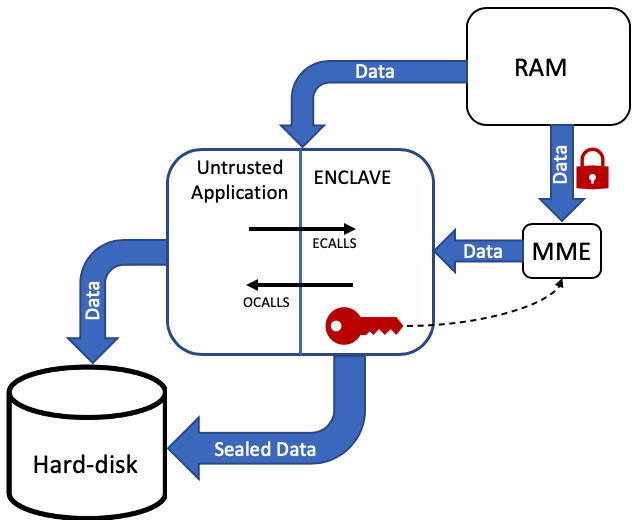
\includegraphics[width=0.75\textwidth]{images/theoric/memory_sgx}
    
    \caption{SGX Memory Management}
    \label{figure:theoric:memory_sgx}
\end{figure}
\par Memory Management inside an Enclave may sound complicated but the main idea is straightforward: every data exiting or entering the secure world of an Enclave must be encrypted as can be seen in Figure \ref{figure:theoric:memory_sgx}. The information inside an Enclave is stored inside the EPC (Enclave Page Cache) which uses the MME (Memory Encryption Engine) to encrypt the pages. This MME is a new and dedicated chip for this purpose. This means that reading information on the memory bus will only result in observing raw encrypted data. The EPC can only be decrypted inside the processor core thanks to keys generated at the Enclave creation.

\subsubsection{Trust establishment}
\label{section:theoric:trust_establishment}
\par For an Enclave to establish trust, there are three main activities:
\begin{itemize}
    \item \textbf{Enclave Measurement:} Enclaves are accompanied with a self-signed certificate provided from the enclave author allowing the Enclave to detect whether any portion of the Enclave code has been tampered with. Unfortunately, this is not enough as it only authenticates the initial state of the Enclave, not the running state. To cope with this, two more information are provided within the certificate.
    \par First, a measurement 256-bit hash that identifies the code and the initial data loaded inside the Enclave. When the Enclave code and data pages are placed inside the EPC, the CPU calculates this measurement. Second, there is also a hash of the Enclave Author's Public Key. This last information allows enclaves authenticated with the same public key to securely speak to each other.
    \item \textbf{Data sealing:} When an enclave is instantiated, as discussed above, its data and code are protected inside the Enclave. Unfortunately, they can't stay forever, when the Enclave stops, it must be able to encrypt these pieces of information into untrusted storage. This process is called the sealing procedure and in most cases, the untrusted storage is the hard-disk of the computer. SGX Enclaves use a sealing key that can be derived even if the Enclave is stopped at some point in time. There are two manners to derive it: either using the Enclave Identity (the Enclave measurement) or by using the Signer Identity (the hash of the Enclave Author's Public Key). In both cases, two distinct enclaves will derive two different keys. The main difference is that by using the Signer Identity, two versions of an Enclave share the same key and thus can read the sealed data of each other. On the contrary, using Enclave Identity, the above operation is impossible but it may be an advantage, as it disables the migration of data between multiple Enclaves.
    \item \textbf{Enclave attestation:} An Enclave may need to prove to a third party that it is legit. Intel developed two ways: either local attestation (to another process on the same computer) or remote attestation (to a remote server). We will only focus on the latter attestation procedure as the first one is not relevant in our work. To prove its identity, an Enclave produces a so-called quote which is a credential that reflects the enclave state. This can be done thanks to an architectural Enclave build by Intel called the Quoting Enclave (QE). This quote can then be verified by Intel web-service to check its authenticity. A quote is composed of many information including the Enclave measurement, user-defined data and others. All of this is powered by an anonymous algorithm known as the Intel(R) Enhanced Privacy ID (Intel(R) EPID). This custom scheme allows using a single private key to verify the authenticity of any number of signers in a group (which each uses a different private key). This process implies that the verifier doesn't know which member of the group signed a quote but can verify its correctness. Obviously, in the SGX context, this EPID group is the collection of SGX enabled platforms.
\end{itemize}

\end{document} 